\section{Lexical analyzer}
\label{Lexical analyzer}

The lexical analyzer\footnote{Implemented in module \texttt{lexical\_analyzer.c} with the corresponding header file \texttt{lexical\_analyzer.h}}, implemented as a finite-state machine (\ref{fsm_diagram}), decomposes source code from standard input into a sequence of tokens. Individual tokens are represented by the final states.

\subsection{Implementation}
When the automaton is in the final state and is not able to process the input char, it returns a token to the parser. When the automaton is not in the final state and is not able to process the input char, it returns a lexical error.
Each state is represented by a function. The current state is stored in a global variable as a pointer to the corresponding function. Each states sets the function pointer to the next state using the \texttt{NEXT\_STATE} macro, depending on the loaded char.
The token is represented by a structure containing information about the token type, value and flag that indicates the presence of \texttt{EOL} before the processed token. Token value is implemented as a \texttt{union} and can contain the name of an identifier, an int, string or double literal value or a boolean \texttt{is\_nilable}. The token type is implemented using the enum type.

The main loop performs a passage through the automaton by repeated invocation of the function referenced by the variable.
Additional global variables, that help remember information that have a lifetime longer than one state, are added in the lexical analyzer.
The communication interface with the lexical analyzer is implemented using the function \verb|get_token()|, which has one parameter that represents a pointer to the variable to load the token into.
The Lexical analyzer includes counters (\verb|actual_line| and \verb|actual_column|) to tell where the error occurred.

\newpage

\subsection{Finite-state machine diagram}
\vspace*{\fill}
\begin{figure}[ht!]
\begin{center}
    \label{fsm_diagram}
    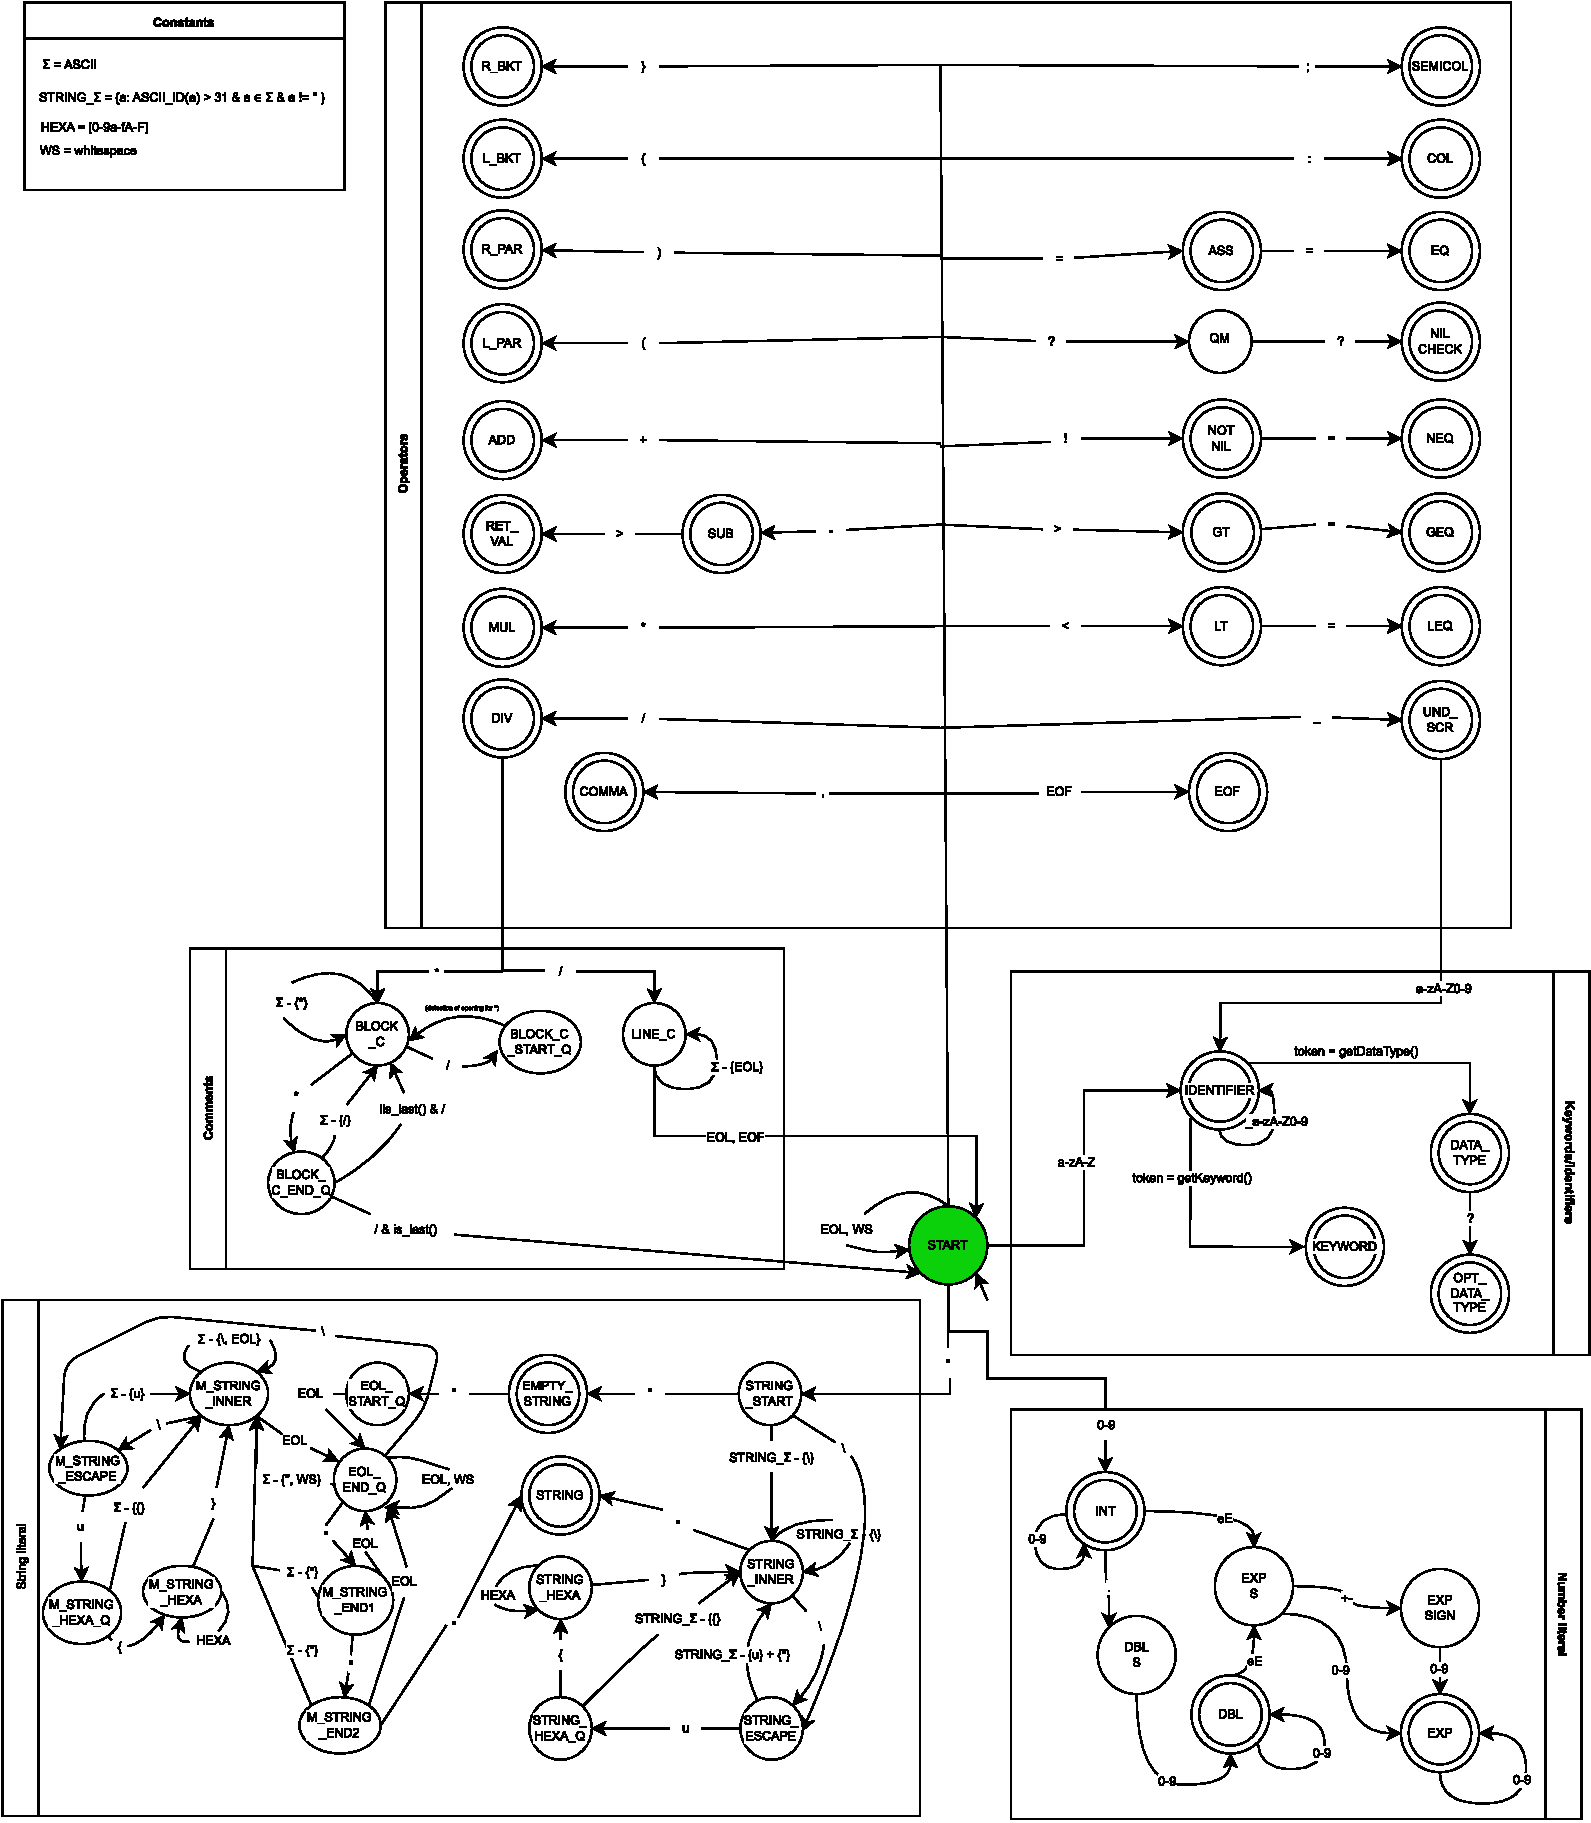
\includegraphics[width=\textwidth, keepaspectratio]{images/fsm_draft.pdf}
    \caption{Finite-state machine diagram}
\end{center}
\end{figure}
\vspace*{\fill}

\newpage